\indent

The main goal  for J/$\Psi$ electroproductionis to study t-dependence of the cross section for different Q$^2$ ranges. In order to calculate acceptances, cross sections, and the rates, coverage in kinematics is studied for events when electron, $\mu^+$ and $\mu^-$ are detected, and electron has momentum $p>0.5$ GeV/c. In Fig.\ref{fig:jp_e0p5_q2w} Q$^2$ vs W (total invariant mass) is shown. Because of rather limited energy range, we will integrate the full W-rage for a given Q$^2$ bin. So the future selection proceeds for W-range $4.025 < W < 4.525$ GeV.   

\begin{figure}[htbp]
\begin{center} 
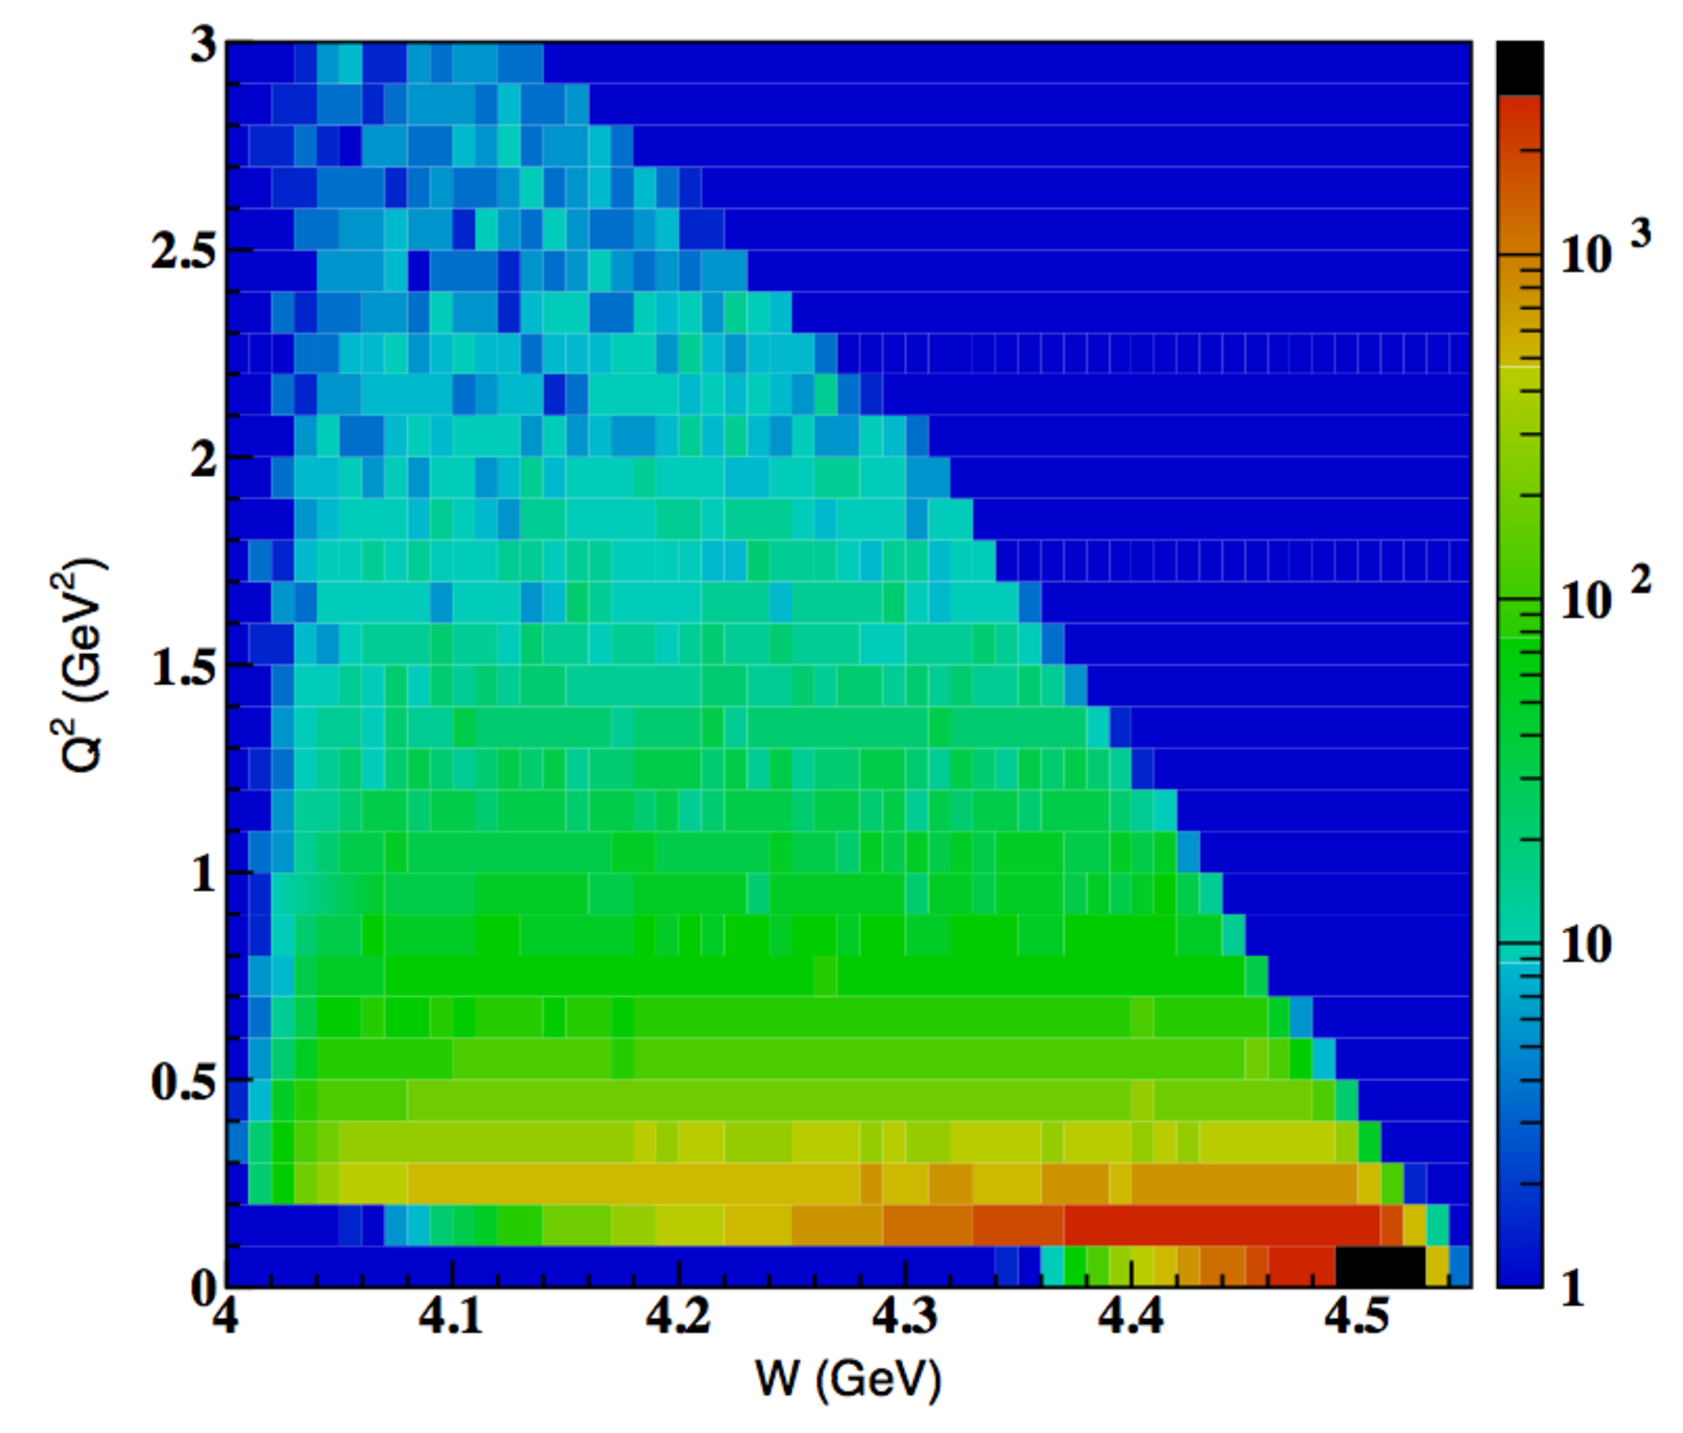
\includegraphics[width=0.8\textwidth]{jpsi_q2_w_emin_0p5.pdf}
\caption{Q$^2$ vs. W  dependance for events with electron, and both muons detected. There is $0.5$ GeV/c minimum momentum cut for the electrons.}
\label{fig:jp_e0p5_q2w}
\end{center}
\end{figure}

\begin{figure}[htbp]
\begin{center} 
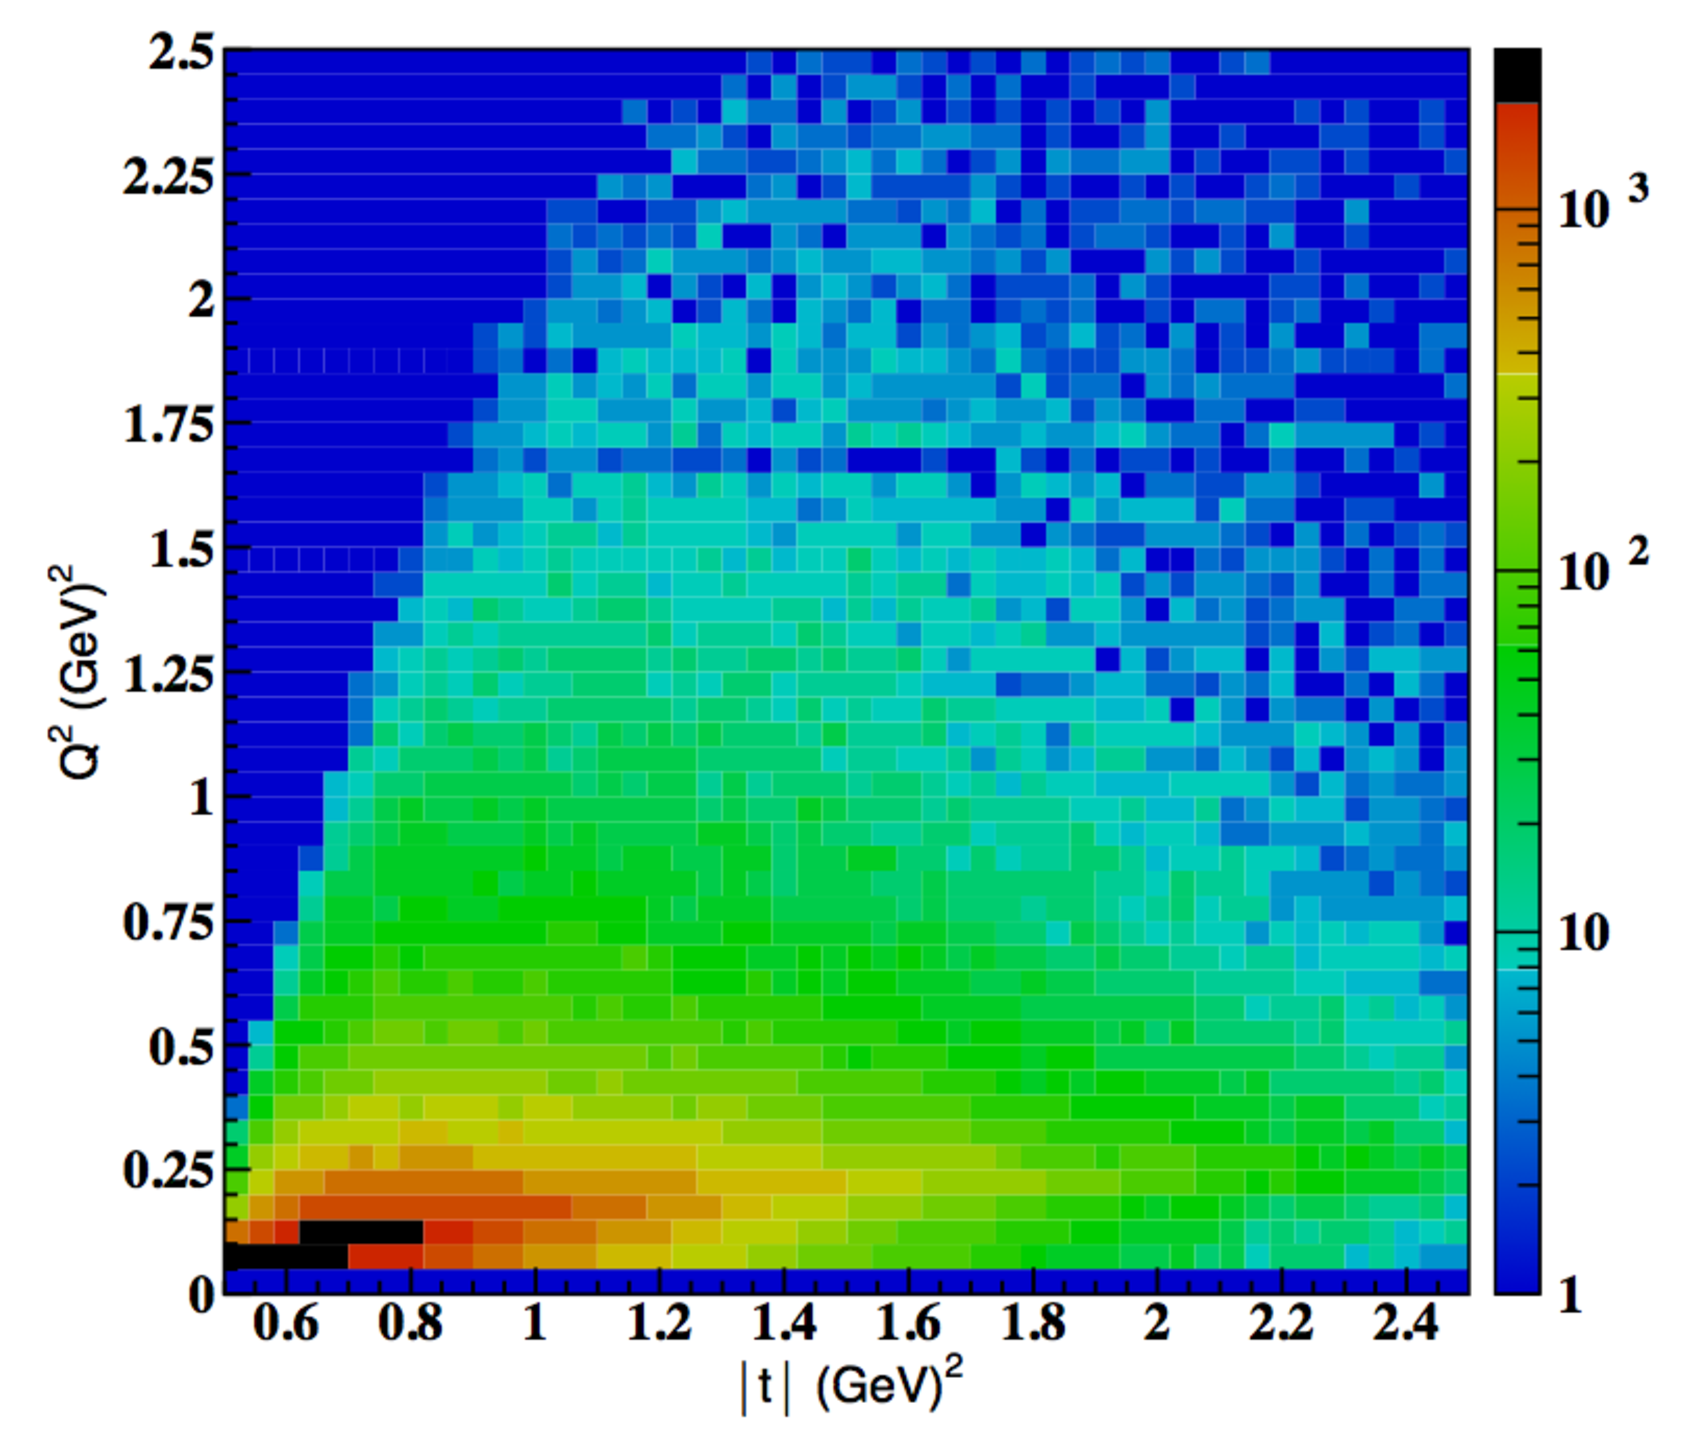
\includegraphics[width=0.8\textwidth]{jpsi_q2_t_w4025_w4525.pdf}
\caption{Q$^2$ vs. t  dependance for $4.025 < W < 4.525$ GeV.}
\label{fig:jp_q2t}
\end{center}
\end{figure}

Fig.\ref{fig:jp_q2t} shows Q$^2$ - t landscape in the selected W-range. Based on this distribution the t-dependance was studied for three bins of Q$^2$, $0.1<$Q$^2 <0.3$ GeV$^2$, $0.3<$Q$^2 <1.$ GeV$^2$, and $1<$Q$^2 < 2.5$ GeV$^2$. The average values of Q$^2$ in each bin are $0.19$ GeV$^2$,  $0.5$ GeV$^2$, and $1.45$ GeV$^2$, respectively. For these studies cross sections are calculated using bin average values for W, Q$^2$, and $t$.


\subsubsection{Cross Section Formalism.}
\indent

The cross section of $t$-channel meson electroproduction on the
nucleon (see diagram on Figure \ref{fig:diagn}), integrated over the
azimuthal angle between electron and hadron planes, can be presented 
as a sum of cross sections for transversely ($\sigma_T$), and
longitudinally ($\sigma_L$) polarized photons: 
\begin{eqnarray}
\label{eq:cse}
{d\sigma _{eN \rightarrow eM^0 N}  \over dQ^2dWdt}=
\Gamma_W\cdot ({d\sigma_T \over dt}~+~\epsilon{d\sigma_L \over dt}) \ .
\end{eqnarray}
Here $\Gamma_W$ is the flux of virtual photons and is defined as:
\begin{eqnarray}
\label{eq:flux}
\Gamma_W=
{\alpha\over 4\pi}\cdot{W^2-m^2\over m^2E^2}\cdot{W\over Q^2}\cdot 
{1\over 1-\epsilon}  \ .
\end{eqnarray}
In the equations above, $\epsilon$ is the virtual photon polarization and is
given by:
\begin{eqnarray}
\label{eq:eps}
\epsilon = \left( 1+2{Q^2+q^{02}\over 4EE'-Q^2} \right)^{-1} \ .
\end{eqnarray}
%%%%%%%%%%%%%%%%%%% Figure : Fdia %%%%%%%%%%%%%%%%%%%%%%%
\begin{figure}[htbp]
\begin{center} 
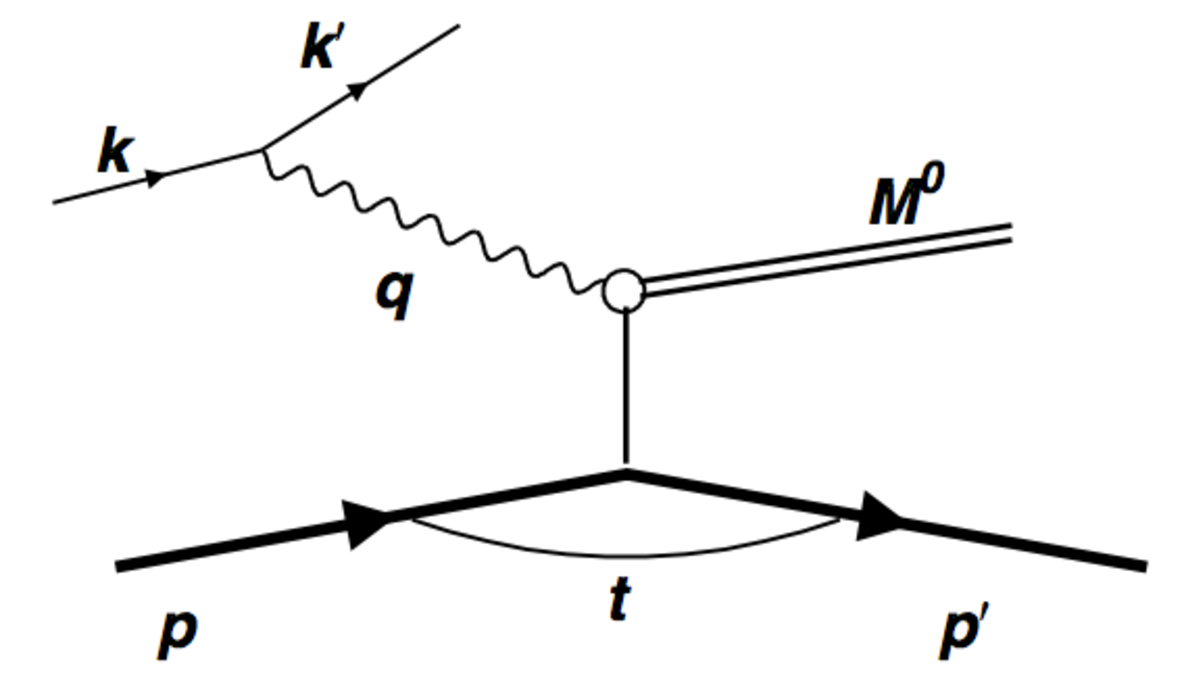
\includegraphics[width=0.7\textwidth]{ep_pm0.pdf}
\caption{Diagram for electroproduction of a $t$-channel meson on the nucleon.}
\label{fig:diagn}
\end{center}
\end{figure}
%%%%%%%%%%%%%%%%%%%%%%%%%%%%%%%%%%%%%%%%%%%%%%%%%%%%

The other kinematical variables are: electron transfered momentum squared
$Q^2=-q^{\mu 2}$ were $q^\mu=(k^\mu-k^{\prime \mu})$ is the four-momentum 
of the virtual photon, and $k^\mu$($k^{\prime\mu}$) is the 
four-momentum of incoming (outgoing) electron. In Eq.(\ref{eq:cse}) $t$
is the transferred momentum squared to the target, and the mass squared 
of the virtual photon hadron system, $W^2$, is:
\begin{eqnarray}
\label{eq:w}
W^2~=~m^2+2mq^0 - Q^2 \ ,
\end{eqnarray}
$m$ is the nucleon mass.

Using vector meson dominance (VDM) one can relate $\sigma_T$
and $\sigma_L$ to the photoproduction cross section \cite{vdm}.
The relation for $\sigma_T$ is:
\begin{eqnarray}
\label{eq:st}
\sigma_T ~=~  \left( {m_{J/\Psi}^2\over 
m_{J/\Psi}^2+Q^2} \right) ^2\cdot \sigma_{\gamma N \rightarrow M^0N} \ ,
\end{eqnarray}
and for $\sigma_L$:
\begin{eqnarray}
\label{eq:sl}
\sigma_L~=~\left( {m_{J/\Psi}^2\over m_{J/\Psi}^2+Q^2} 
\right) ^2\cdot 
{Q^2\over m_{J/\Psi}^2}\cdot (1-x)^2
\cdot \xi(Q^2,\nu)\cdot \sigma_{\gamma N \rightarrow M^0p} \ ,
\end{eqnarray}
where $m_{J/\Psi}$ is the $J/\Psi$ meson mass. 
$\xi(Q^2,\nu)$ scales the model to the data, and is taken to be $0.5$ for our calculations.  
The $x=Q^2/(2qp)$ where $p$ is the four-momentum of the target nucleon. 
The $\sigma_{\gamma N
\rightarrow M^0N^\prime}$ is the photoproduction cross section. For our calculations we used 2-gluon formalism for the differential cross section from \cite{brodsky:2000zc}:

\begin{eqnarray}
{d\sigma\over {dt}} = N_{2g}\nu{(1-x)^2\over{R^2M^2}}F^2_{2g}(t)(s-m_p^2)^2
\end{eqnarray}
where where $F_{2g}(t)$ is the proton form factors that take into account the fact that the three target quarks recombine into the final proton after the emission of two gluons. The $N_{2g}$ is scaling factor to saturate measured cross sections, $M$ is the mass of the $c\bar c$, $R$ is the proton radius (taken as $1$ fm, $s$ is the center mass energy square and the $x$ is the fraction of the proton momentum carried by the valence quark.  

\begin{figure}[htbp]
\begin{center}
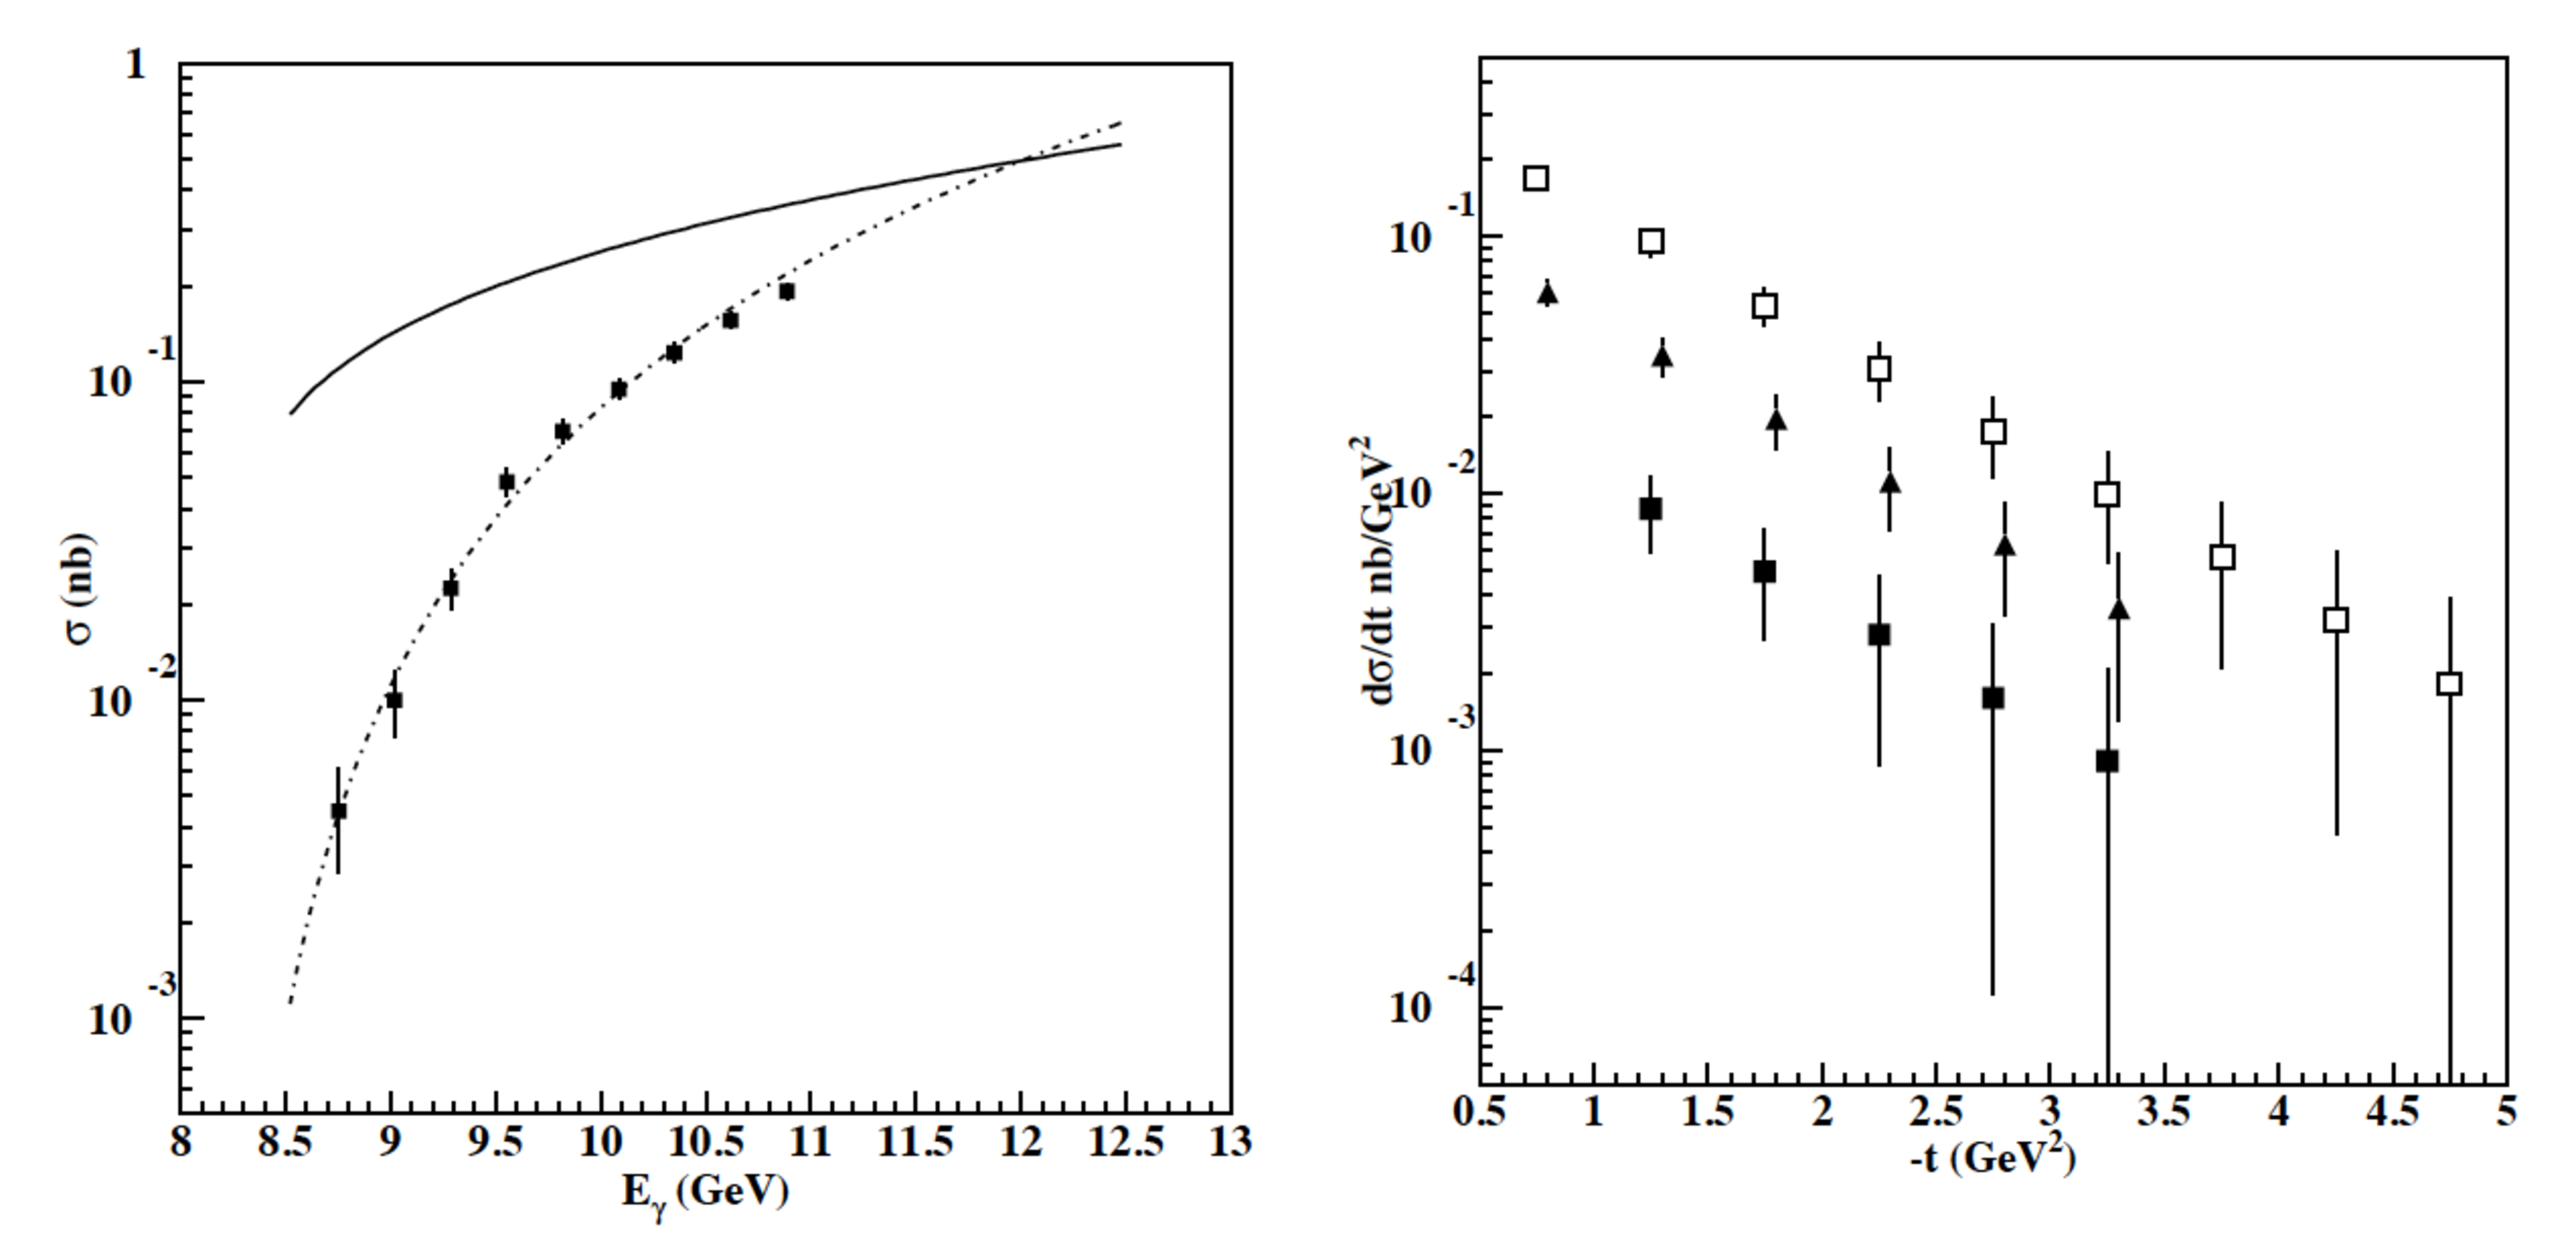
\includegraphics[width=1\textwidth]{jpsi_photo.pdf}
\end{center}
\caption{The cross section of exclusive $J/\psi$ photoproduction in 100 days of running from \cite{tcs_clas12}. On the left: total cross section as a function of the incoming photon energy. The curves are calculated according to cross section formulas in Ref. \cite{brodsky:2000zc}. On the right: Differential cross section as a function of the four-momentum transfer $-t$ for three bins of $s$. The dashed line and the filled squares are for $s=17.55$ to $18.05$ GeV$^2$, the dotted line and the inverted filled triangles are for $s=19.05$ to $19.55$ GeV$^2$, and the dashed-dotted line and the open squares are for $s=21.05$ to $21.55$ GeV$^2$.}
\label{fig:jpsixs2}
\end{figure}


This cross section model has been used to calculate cross sections for the experiment E-12-12-001 \cite{e1212001}. The $t$-distribution for exclusive $J/\Psi$ photoproduction from E12-12-001 proposal is shown in Fig.~\ref{fig:jpsixs2}. The same code was used to calculate cross sections for the electroproduction cross section in the kinematics of the present proposal.


\label{acc_simulations}
\indent


\clearpage

\subsubsection{Acceptance simulations for J/$\Psi$}
\indent

The generator used for J/$\Psi$ acceptance studies simulates multi-particle final states in photo- and electro production reactions. It has correct decay channels and branching ratios for most of particles listed in PDG (Lund/Jetset \cite{lepto}) and allows to set the kinematic dependencies, e.g. Q$^2$ and $t$. The reaction: 
\begin{eqnarray}
ep\to e^\prime~J/\Psi~p^\prime\to e^\prime\mu^+\mu^-p^\prime
\end{eqnarray}
was simulated with the following conditions:
\begin{itemize}
\item beam energy $E=11$ GeV
\item electron four momentum transferred dependence $1/{Q^4}$ ($Q^2=-q^2=-(k_i-k_f)^2$, where $k_{i(f)}$ is the initial (final) four momentum of the electron)
\item exponential dependence for the squared four-momentum transfer from initial to final state proton, $e^{3t}$, ($t=(p_i-p_f)^2$, where $p_i$ and $p_f$ are four momenta of the initial and final state protons)
\end{itemize}

The Q$^2$- and t-dependences as they have been generated initially and their form after the electron is selected in the calorimeter detection range are shown in Fig.\ref{fig:jp_sim}. The cutoff on maximum Q$^2$ and t after electron selection are due to the minimum momentum, $p_{min}=0.5$ GeV, and the maximum angel, $\theta_{max}=35^\circ$ limits.

\begin{figure}[htbp]
\begin{center}
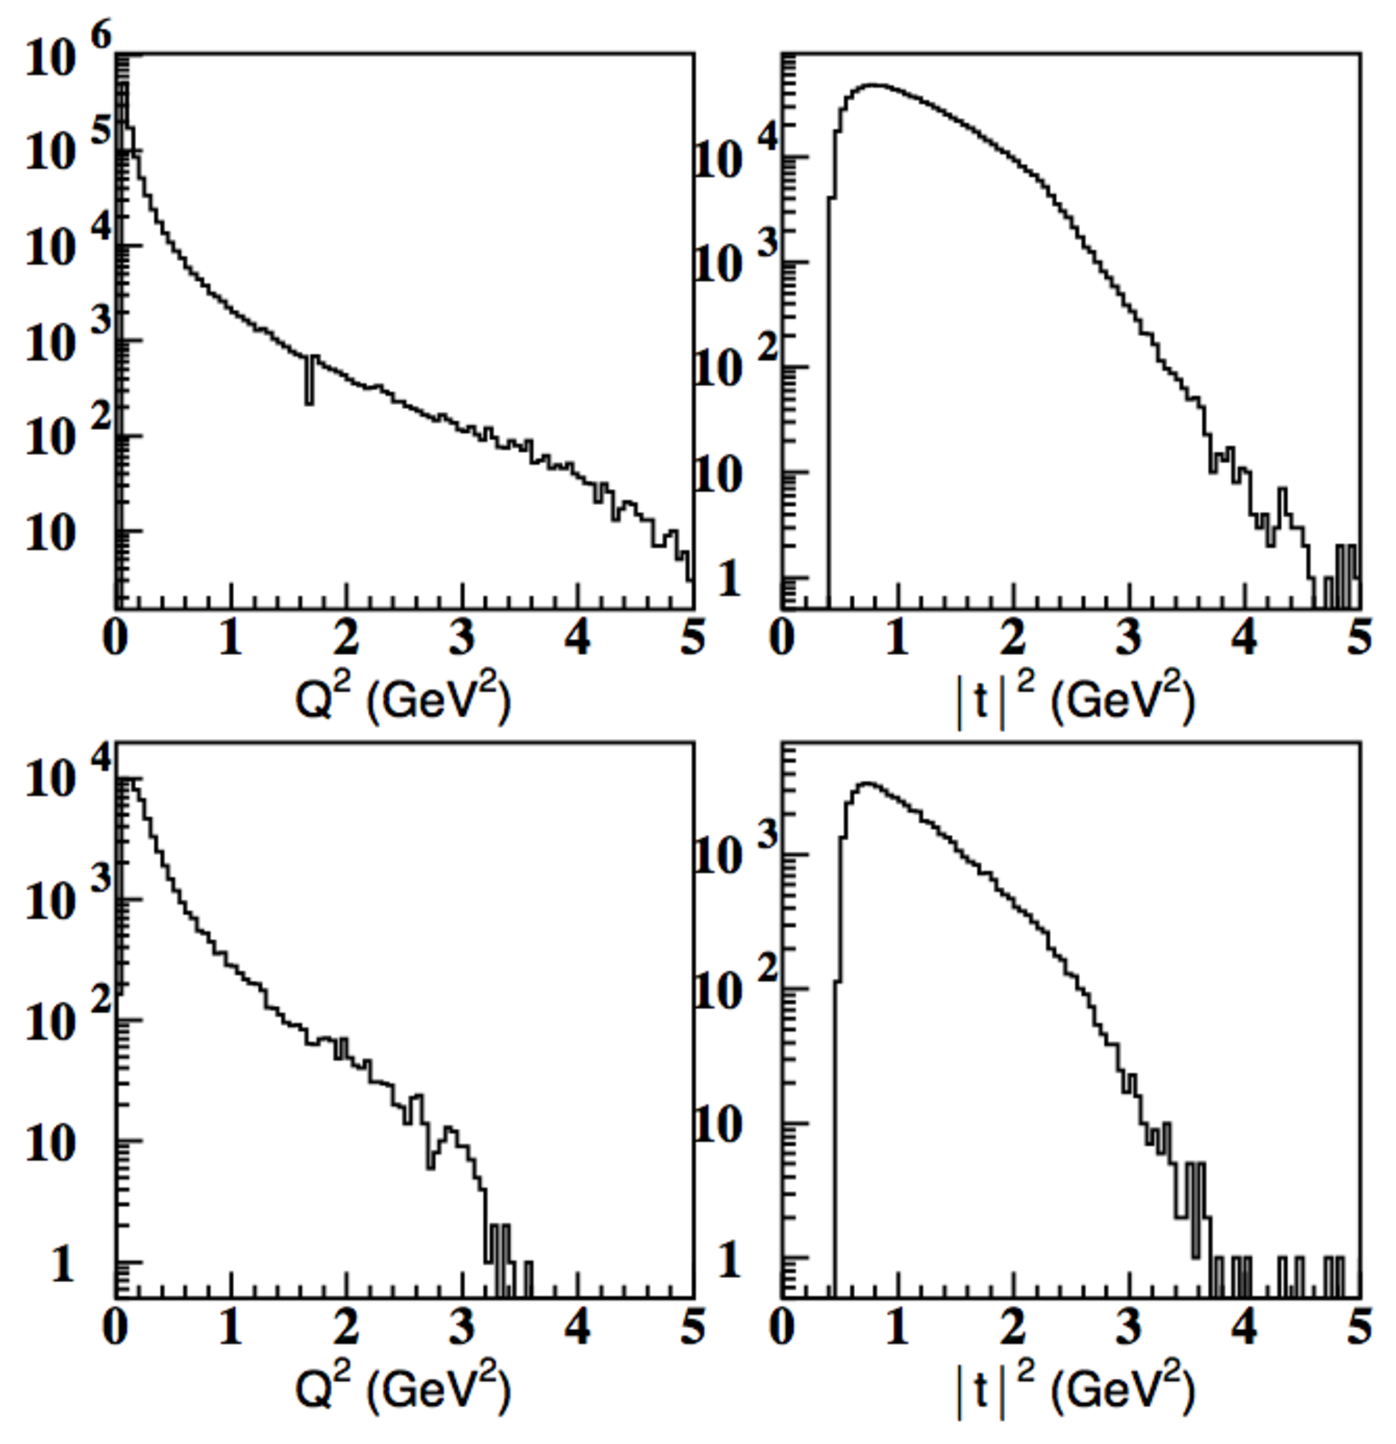
\includegraphics[width=0.8\textwidth]{jpsi_q2_t_sim.pdf}
\caption{Simulated Q$^2$ and $t$ distributions, top. On the bottom panels the same distributions when electron is detected in the calorimeter.  }
\label{fig:jp_sim}
\end{center}
\end{figure}

In Fig.\ref{fig:jp_kine}, momentum vs. scattering angle distributions for final state particles in the reaction $ep\to e^\prime p^\prime J/\Psi$ are shown. Due to large momentum transfer, near threshold  production, recoil protons will scatter at forward direction and will not be detected. Electrons will be detected in the calorimeter as was described above in the angular rage $5^\circ < \theta_e <35^\circ$ with momentum $p>0.5$ GeV/c. The muons are produced mostly in forward angles ($\theta_\mu<40^\circ$), bottom left panel of Fig.\ref{fig:jp_kine}, and remain in the same momentum-angular space with electrons in the calorimeter, bottom right panel. The CLAS12 FD that can detect changed tracks in angular range $5^\circ < \theta <35^\circ$ is well suited for detecting muons from presented reaction. In Fig.\ref{fig:jp_mukine} momentum vs scattering angle of $\mu^+$ and $\mu^-$ are shown. Due to large momentum there is not much difference in detection acceptance for negatively and positively charged tracks at forward angles due to the magnetic field and the CLAS12 detector acceptances.

\begin{figure}[htbp]
\begin{center}
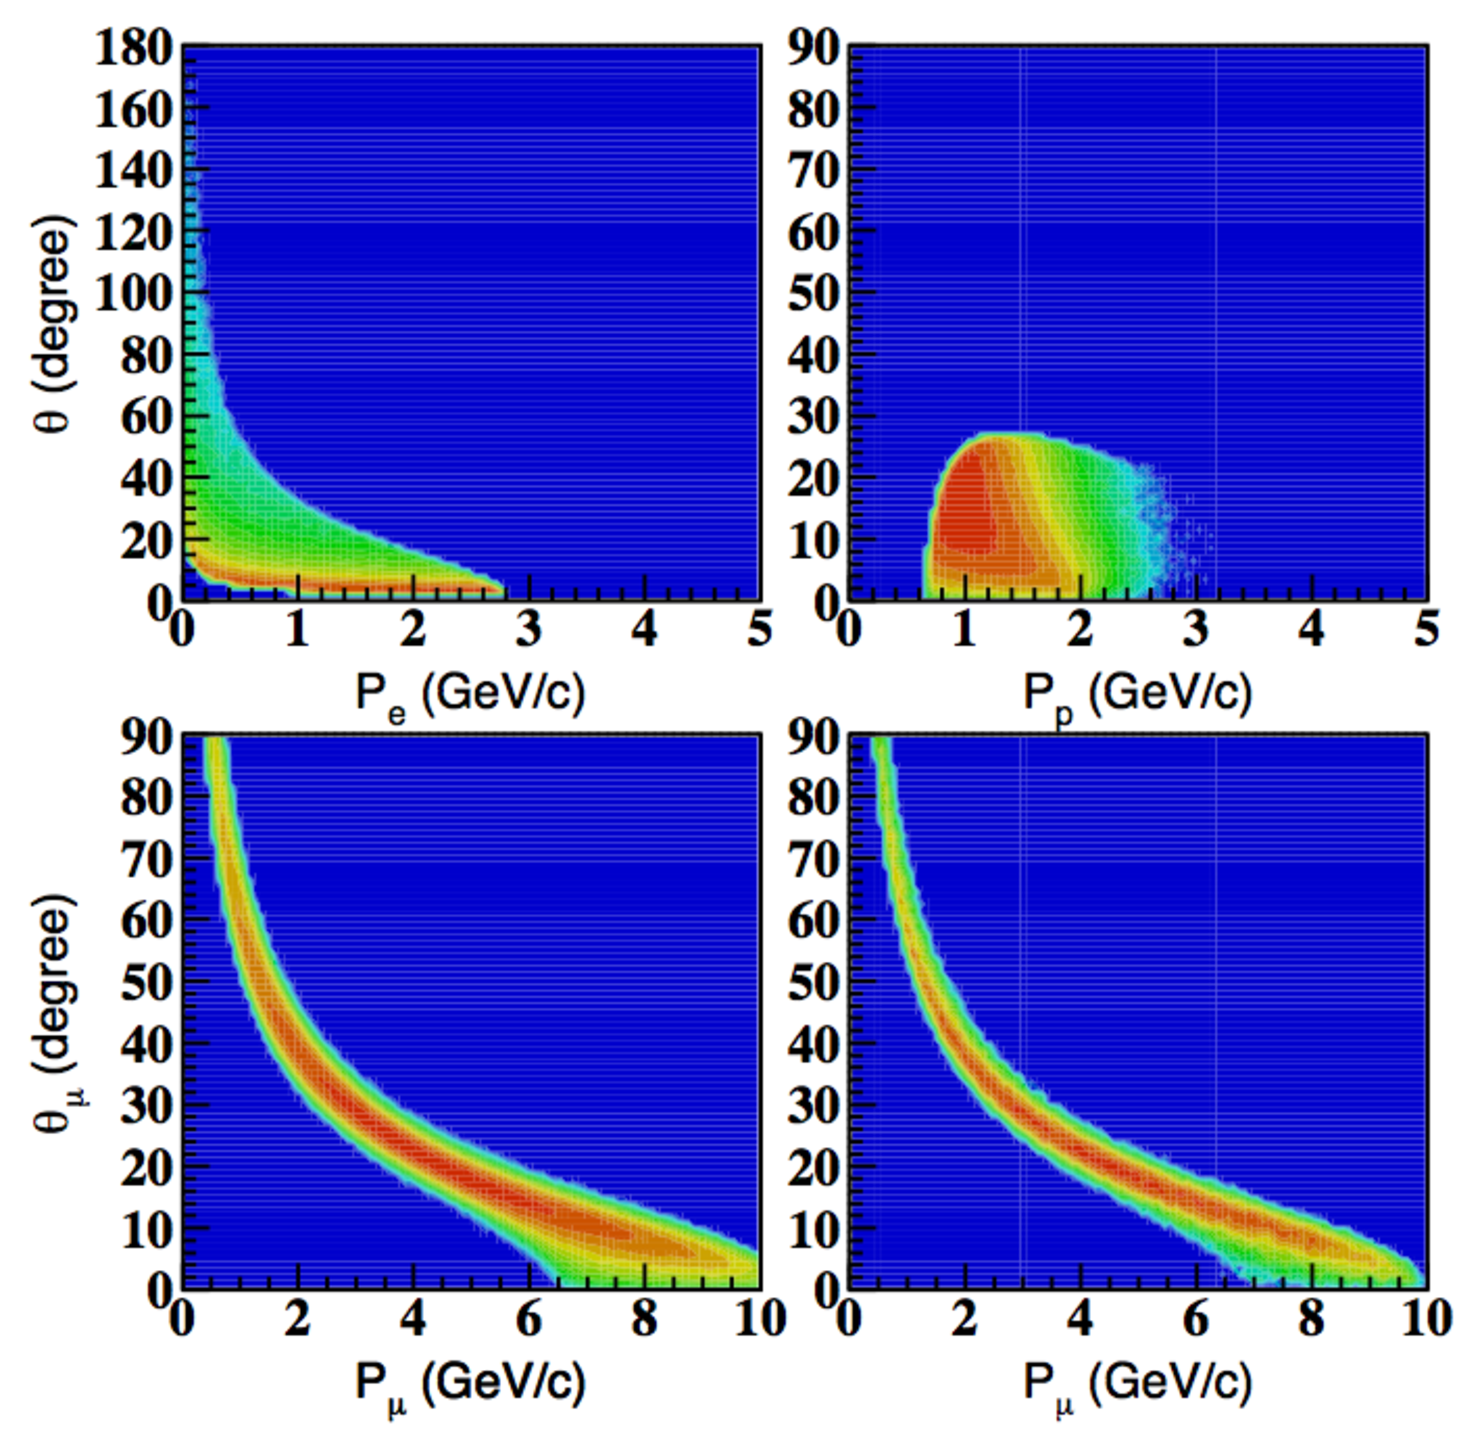
\includegraphics[width=0.8\textwidth]{jpsi_kine.pdf}
\caption{Kinematics of the scattered electron, recoil proton, and the decay muons for the reaction $ep\to e^\prime p^\prime J/\Psi $. In the bottom-right panel angular-momentum distribution of muons is shown for events where electron momentum is $p>0.5$ GeV and is in the scattering angular range $5^\circ <\theta<35^\circ$.}
\label{fig:jp_kine}
\end{center}
\end{figure}

\begin{figure}[htbp]
\begin{center}
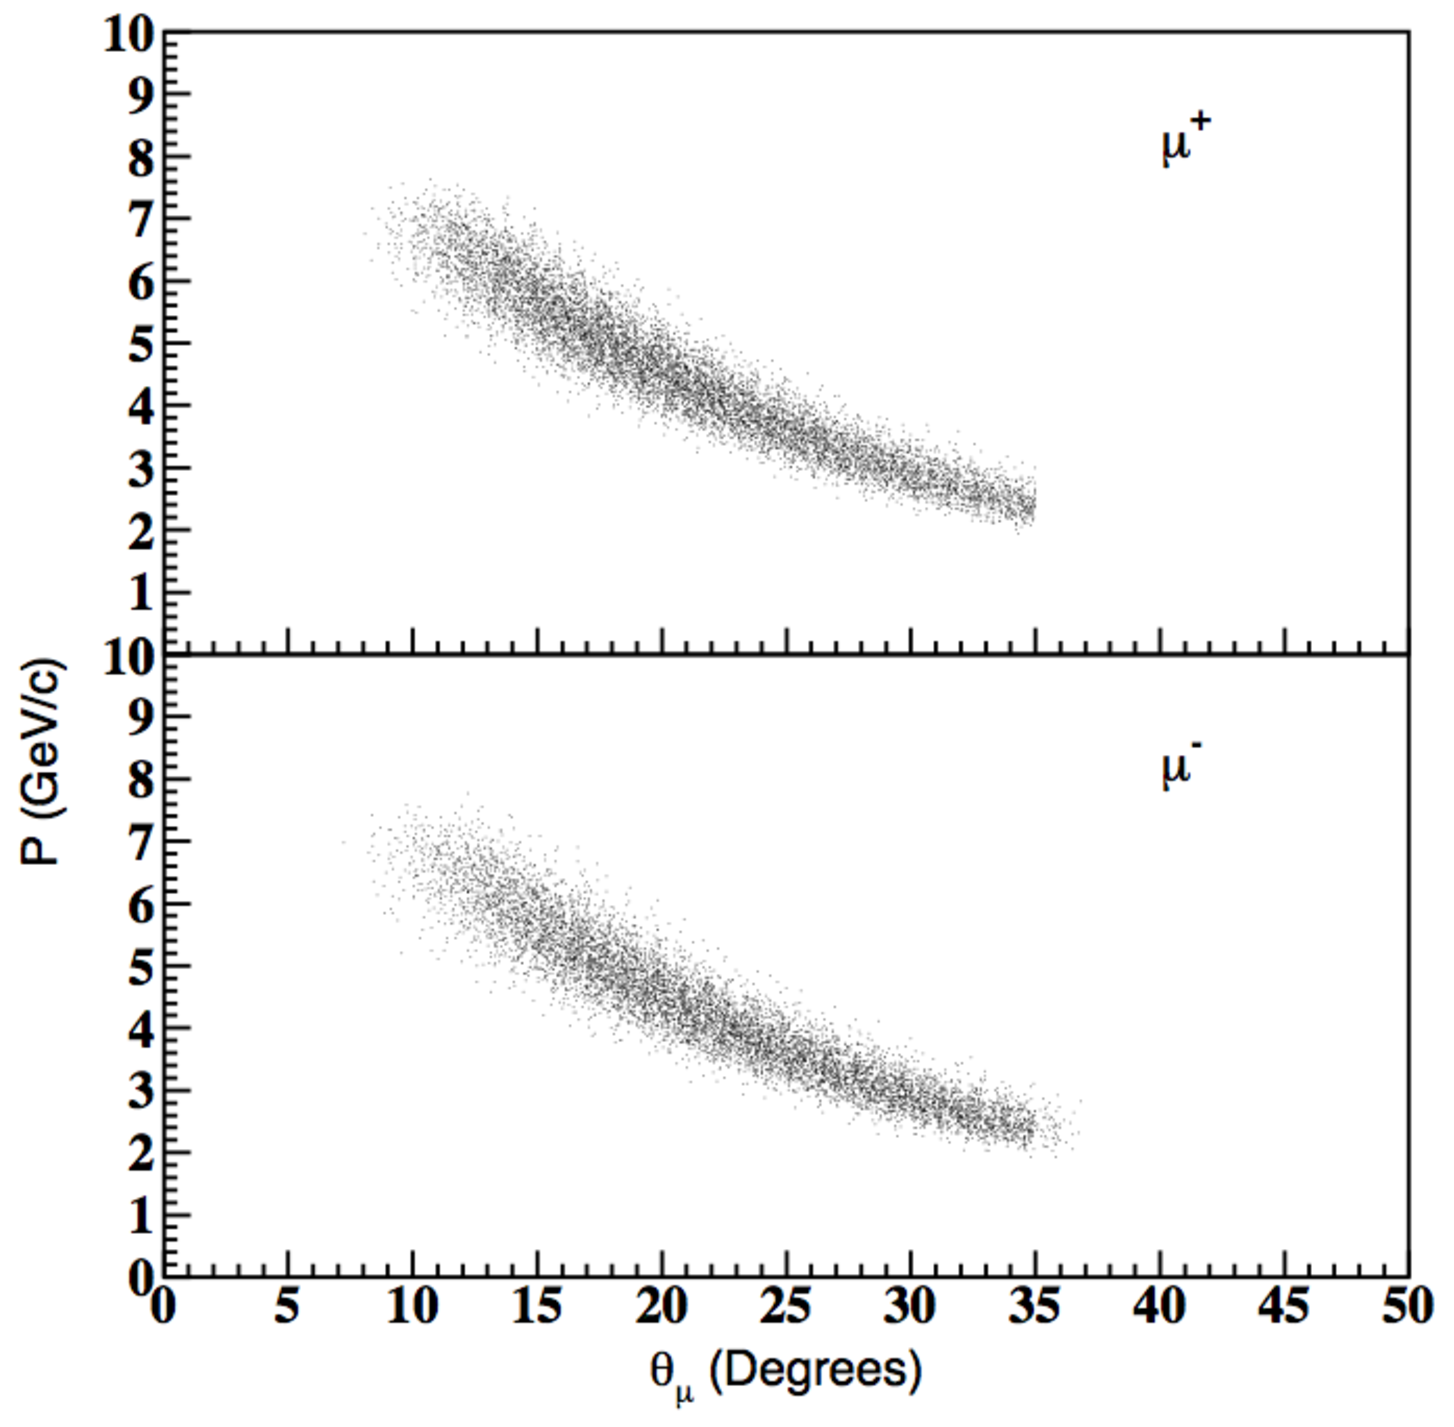
\includegraphics[width=0.6\textwidth]{jpsi_muon_p_theta_detected.pdf}
\caption{Angular-momentum distributions of $\mu^+$ (top) and $\mu^-$ bottom detected in the CLAS12 FD. }
\label{fig:jp_mukine}
\end{center}
\end{figure}

Since the proton will not be detected, when exclusivity is required the missing momentum analysis  of the $e\mu^+\mu^-$ final state will be performed to select events in the reaction $ep\to e^\prime p^\prime J/\Psi$, after identifying the $J/\Psi$ in the invariant mass of the muon pairs. For this, the mass (invariant and missing) resolution  will play an important role in identification of the reaction.  In Fig.\ref{fig:jp_mres} the expected resolutions for invariant and missing masses are shown. These distributions have been calculated using reconstructed, smeared, 3-momenta of the electron, $\mu^+$ and $\mu^-$ using the angular and momentum resolutions described above. Both distributions are fitted with Gaussian function. The standard deviations (mass resolutions) for both are $\sim 47$ MeV, indicating that identification of the J/$\Psi$ or the missing recoil proton is sufficient. 

\begin{figure}[htbp]
\begin{center}
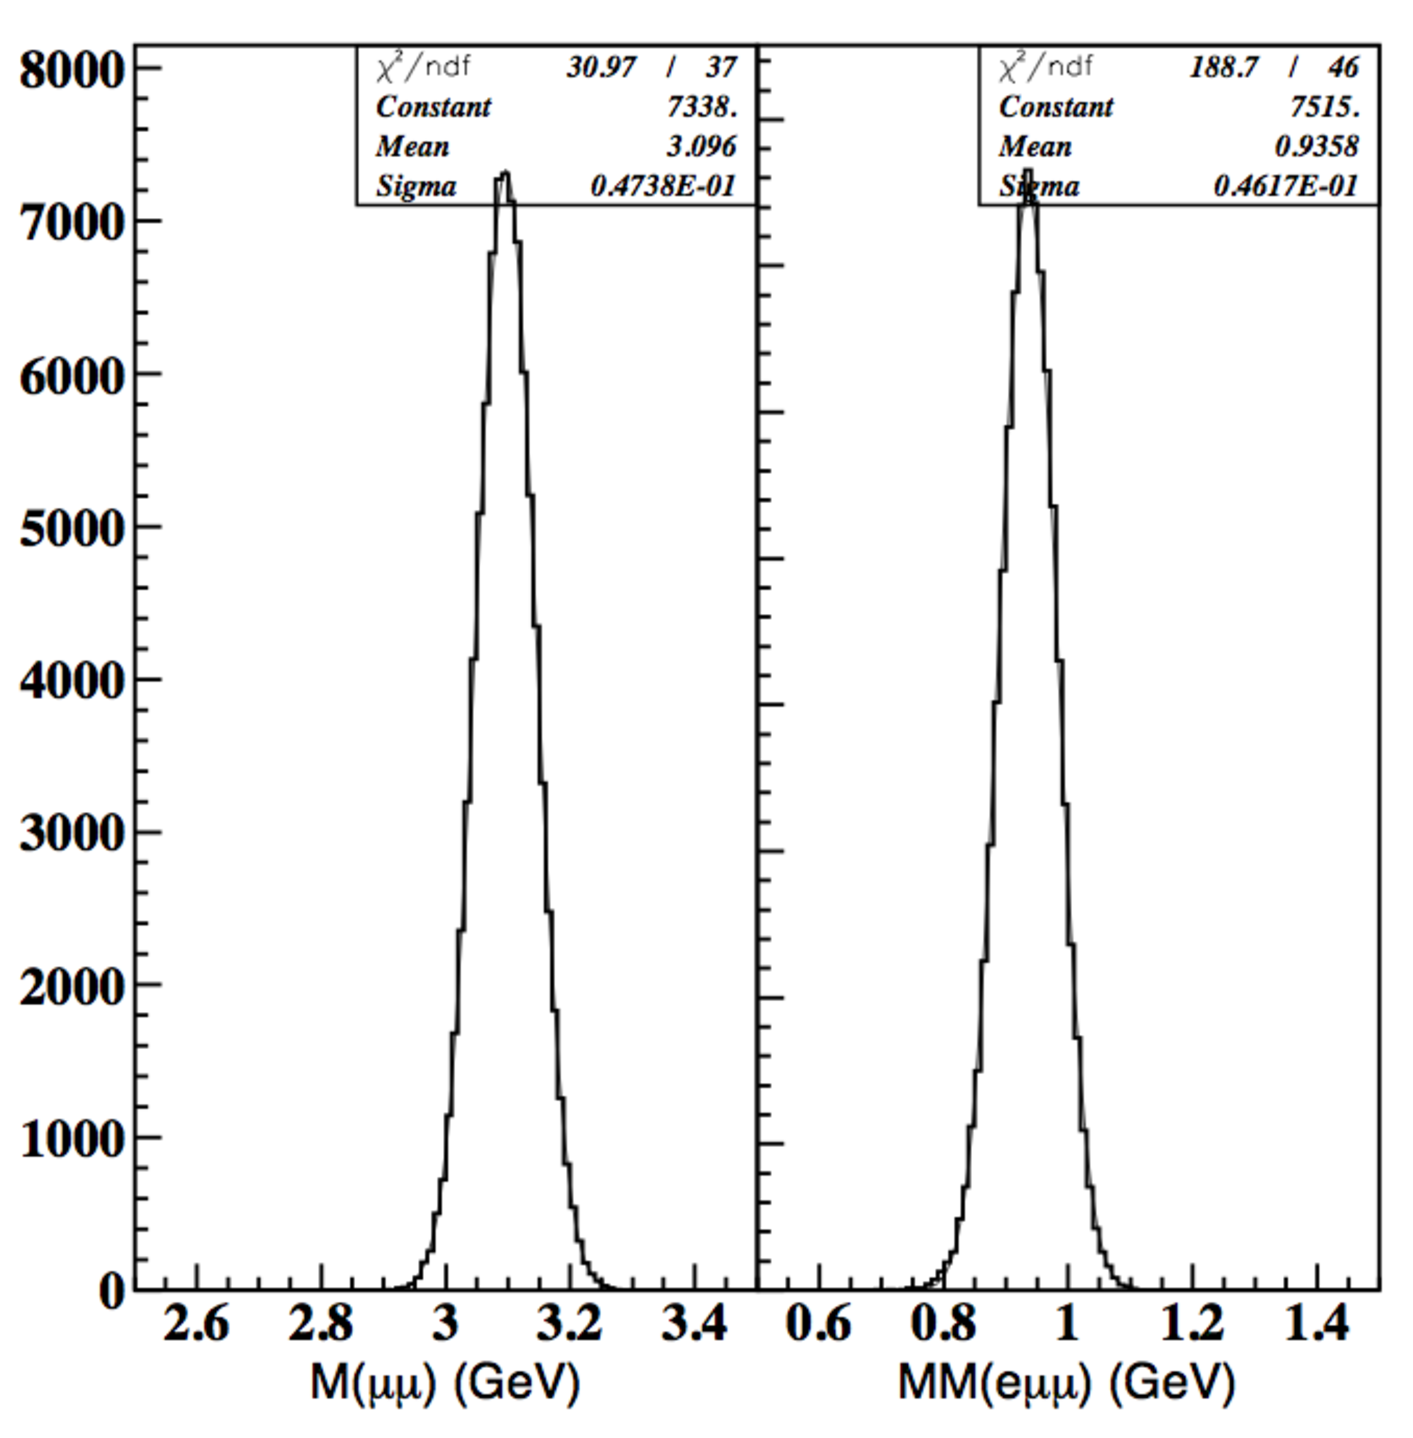
\includegraphics[width=.5\textwidth]{jpsi_minv_mmis_resolutions.pdf}
\caption{Expected mass resolutions: left the invariant mass of muon pairs, right the missing mass squared for the reaction $ep\to e^\prime \mu^+ \mu^- (p)$.}
\label{fig:jp_mres}
\end{center}
\end{figure}

As will be described below, the goal of the J/$\Psi$ electroproduction study will be the measurements of the t-dependence of the cross section in three bins of Q$^2$, $0.1<$Q$^2 <0.3$ GeV$^2$, $0.3<$Q$^2 <1.$ GeV$^2$, and $1<$Q$^2 < 2.5$ GeV$^2$. Therefore, our studies of the acceptances are also in these three bins of Q$^2$. The t-dependence of acceptances shown in Fig.\ref{fig:jp_acc}. The average acceptance for detection of (e$\mu^+\mu^-$) is about $\sim 3\%$, somewhat lower for lowest Q$^2$ bin. These acceptance values are used to calculate expected  rates. 

\begin{figure}[htbp]
\begin{center}
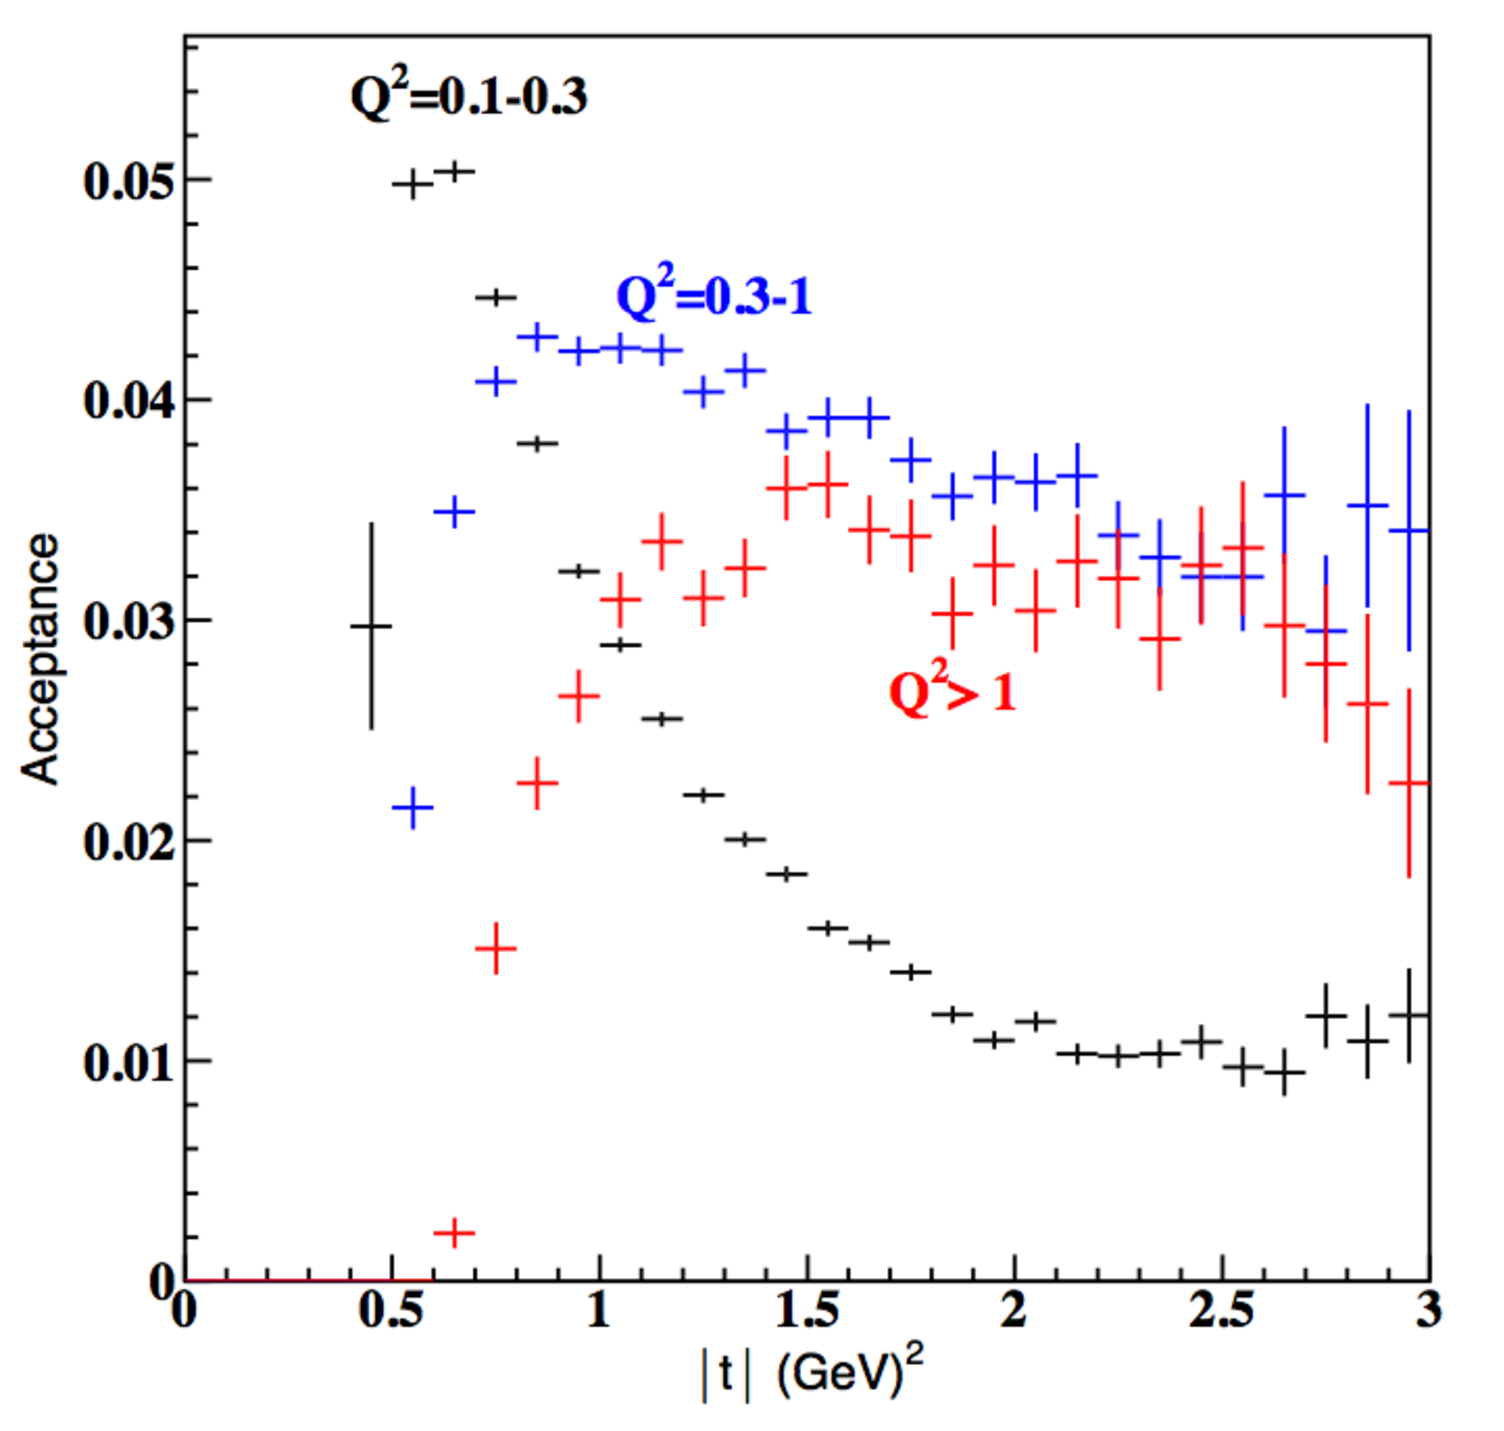
\includegraphics[width=.65\textwidth]{jpsi_t_acceptance_3Q2.pdf}
\caption{Acceptances as a function of $t$ for three Q$^2$ bins.}
\label{fig:jp_acc}
\end{center}
\end{figure}




%\clearpage


\subsubsection{Rates and projected results}
\indent

 Using photoproduction cross sections, $d\sigma/dt$,  from calculations presented in the proposal for the experiment E12-12-001 \cite{e1212001}, first $\sigma_T$ and $\sigma_L$ are calculated as described in Eqs. \ref{eq:st} and \ref{eq:sl}, then the virtual photon flux, $\Gamma_W$ (Eq.\ref{eq:flux}), and the cross section d$\sigma$/dW/dQ$^2$/dt as presented in Eq.\ref{eq:cse} using the bin average kinematical points (W, Q$^2$, and $t$). In Fig.\ref{fig:jp_rates} expected rates as a function of $t$ are shown for three Q$^2$ bins. The projected t-dependances of measured cross section is shown in Fig.\ref{fig:jp_xs}. The error bars on the points are expected statistical accuracy as shown in Fig.\ref{fig:jp_rates}.  
 
\begin{figure}[htbp]
\begin{center} 
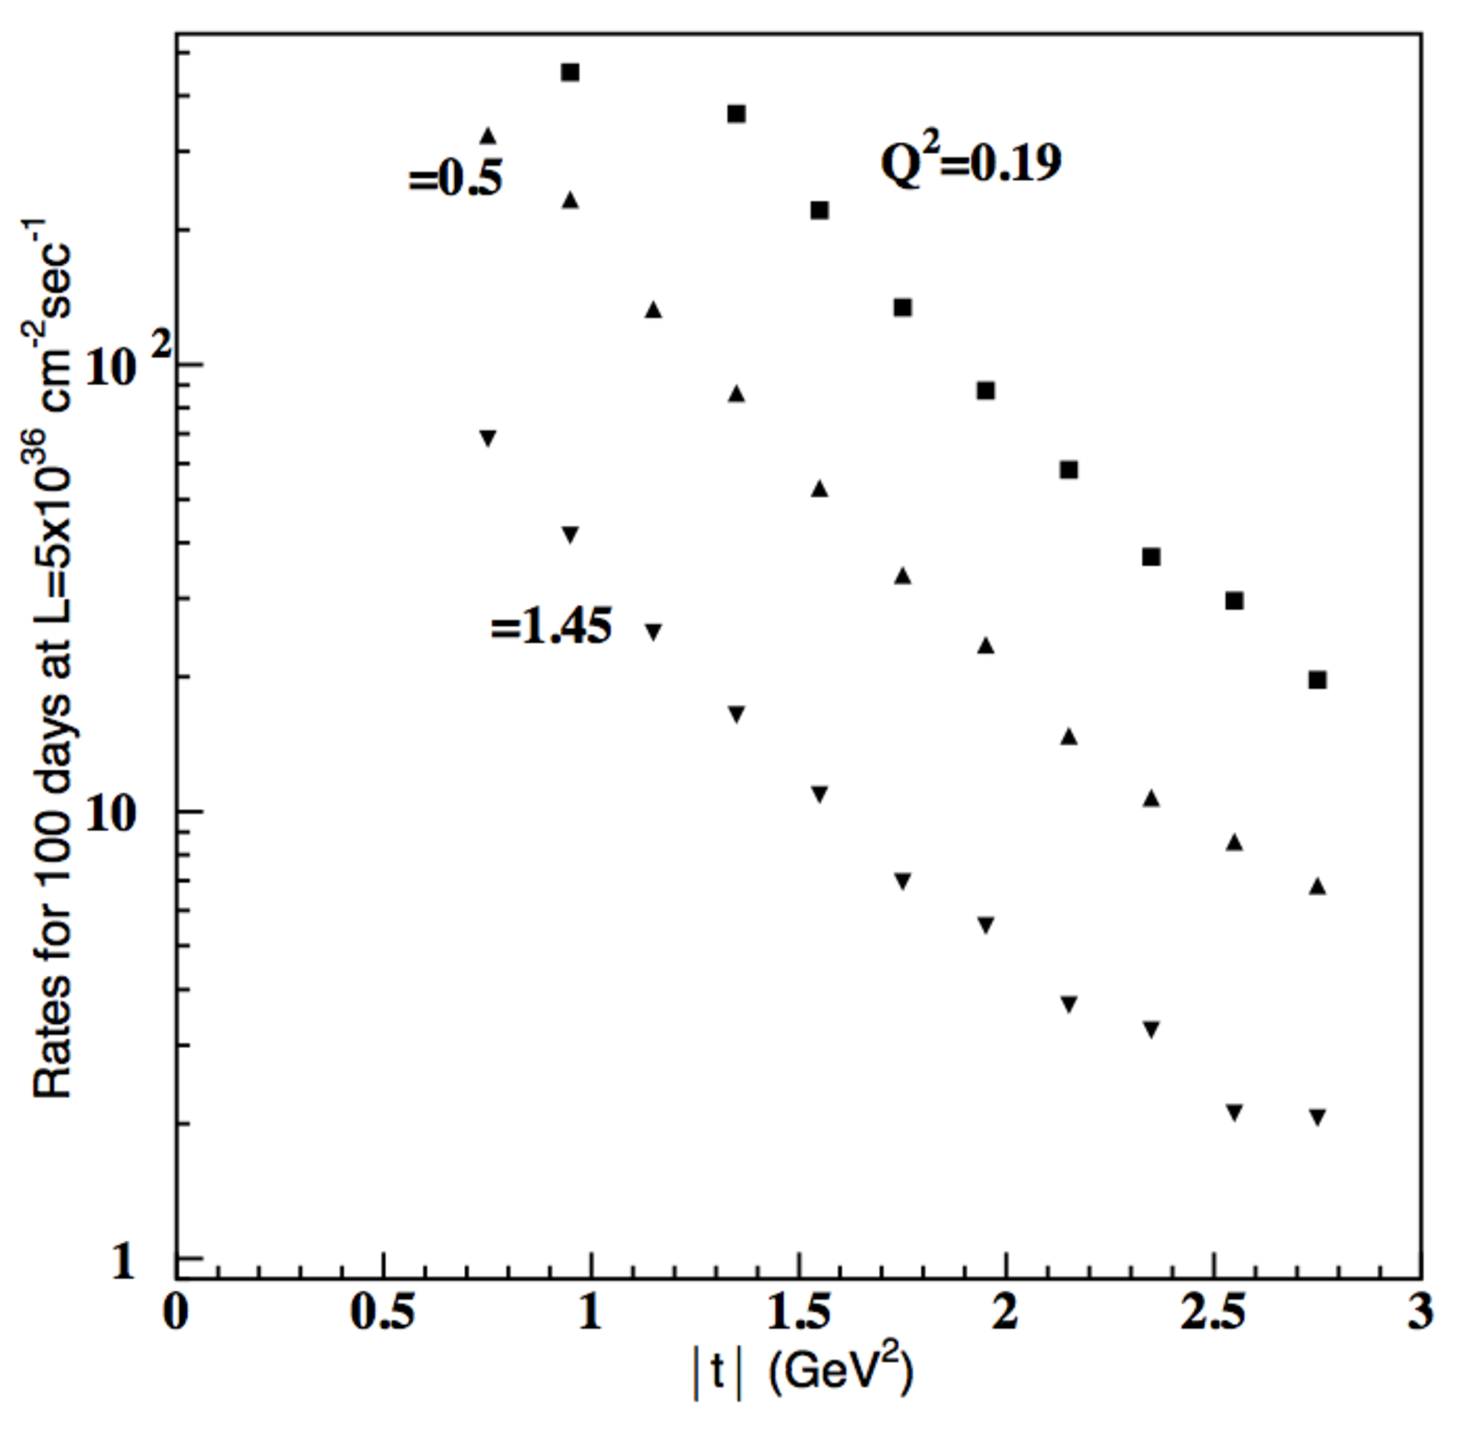
\includegraphics[width=0.65\textwidth]{jpsi_rates_3q2.pdf}
\caption{The expected rates as a function of t  for three Q$^2$ bins for $4.025 < W < 4.525$ GeV. Rates correspond to 100 days of running at luminosity of $5\times10^{36}$ cm$^{-2}$ sec$^{-1}$.}
\label{fig:jp_rates}
\end{center}
\end{figure}

 \begin{figure}[htbp]
\begin{center} 
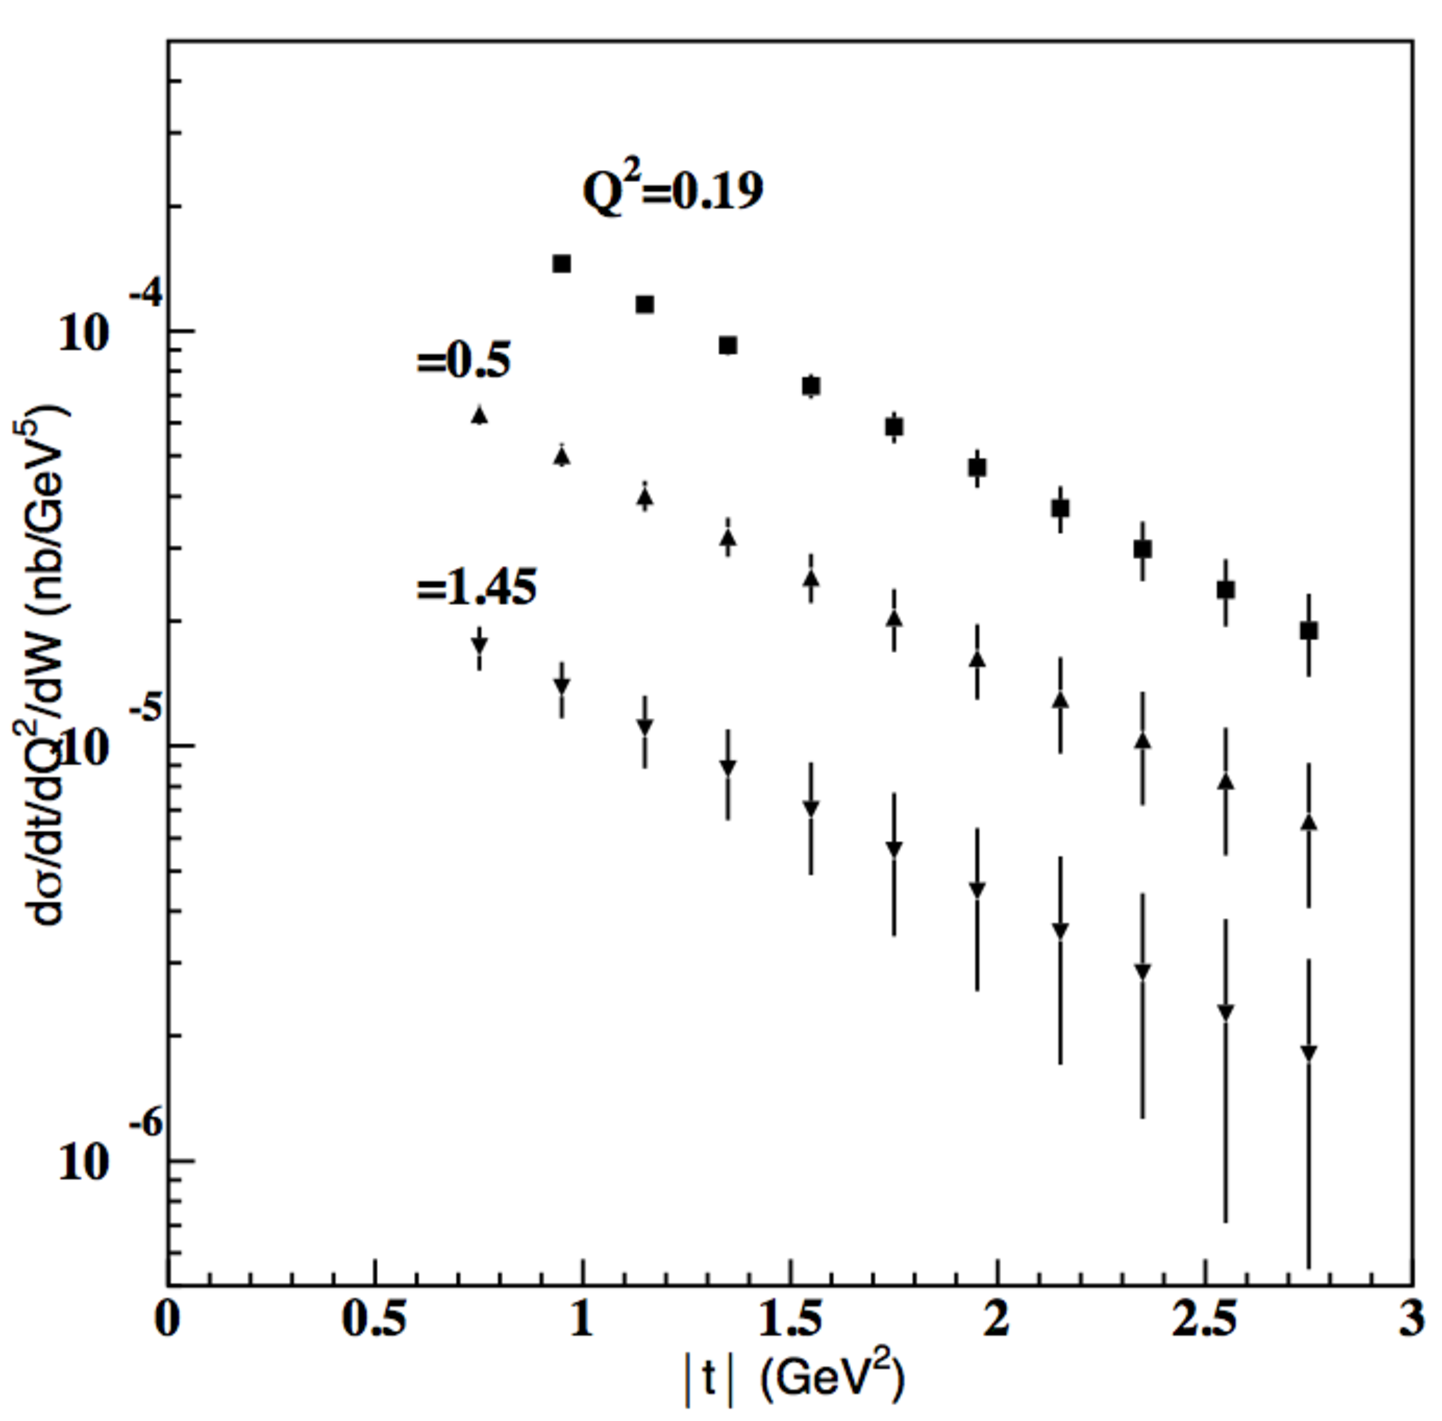
\includegraphics[width=0.65\textwidth]{jpsi_xs_3q2_errors.pdf}
\caption{The expected rates as a function of t  for three Q$^2$ bins for $4.025 < W < 4.525$ GeV. Rates correspond to 100 days of running at luminosity of $5\times10^{36}$ cm$^{-2}$ sec$^{-1}$.}
\label{fig:jp_xs}
\end{center}
\end{figure}


 
 
